\documentclass{article}

\usepackage[utf8]{inputenc}
\usepackage[ngerman]{babel}
\usepackage[ngerman]{translator}
\usepackage[T1]{fontenc}
\usepackage{enumitem}
\usepackage{graphicx}
\usepackage{float}
\usepackage{url}
\usepackage[bottom]{footmisc}
\usepackage{hyperref}
\usepackage[nonumberlist, section=subsection]{glossaries}

\title{\textbf{Entwurf} \\ Cryptographics}
\author{}
\date{\today}

%Glossar-Befehle anschalten
\makeglossaries
% \newglossaryentry{identifier}{name={Name}, description={Description}}

\begin{document}

% The cover page.
\maketitle
\begin{table}[b]
  \begin{tabular}{| l | l | l |}
    \hline
    \textbf{Phase} & \textbf{Verantwortlicher} & \textbf{Email} \\ \hline
    Pflichtenheft & Matthias Jaenicke & matthias.jaenicke@student.kit.edu \\ \hline
    Entwurf & Matthias Plappert & undkc@student.kit.edu \\
            & Julien Duman & uncyc@student.kit.edu \\ \hline
    Implementierung & Christian Dreher & uaeef@student.kit.edu \\ \hline
    Qualitätssicherung & Wasilij Beskorovajnov & uajkm@student.kit.edu \\ \hline
    Präsentation & Aydin Tekin & aydin.tekin@student.kit.edu \\ \hline
    \end{tabular}
\end{table}
\thispagestyle{empty}
\newpage

% Table of contents page.
\tableofcontents
\newpage

% Start of the actual document.
\section{Einleitung}
Für das Kryptologikum des Instituts für Kryptographie und Sicherheit soll die Software Cryptographics zur Demonstration kryptographischer Verfahren erstellt werden. Das Softwareprodukt soll vor allem auf Ausstellungen präsentiert werden und erfordert daher eine möglichst intuitive Benutzerführung.

Um das Ziel der intuitiven Benutzerinteraktion zu erreichen, liegt das Hauptaugenmerk des Entwurfes auf der Planung eines Rahmenwerkes, dass es erlaubt, einzelne Verfahren in die Software einzubetten. Durch wiederverwendbare UI-Komponenten sowie eine einheitliche und für alle Verfahren identischen Benutzerführung erreichen wir dieses Ziel. Zusätzlich erlaubt uns dieser Entwurf, wiederkehrende Aufgaben wie beispielsweise die Soforthilfe mit minimalem Aufwand innerhalb der einzelnen Verfahren zu implementieren. Die eigentliche Komplexität steckt hierbei immer im Rahmenwerk, sodass alle Verfahren von Verbesserungen und Optimierungen profitieren. Weiterhin setzen wir auf eine simples, modulares System, dass es uns erlaubt, Verfahren mit minimalem Aufwand zu implementieren, zu warten und auszutauschen. Grundprinzipien ist hierbei die lose Kopplung der einzelnen Verfahren.

Eine Herausforderung stellte die Abwägung zwischen Konsistenz und einer nötigen Flexibilität innerhalb der Verfahren da. So erfordern beispielsweise unterschiedliche Verfahren durchaus sehr unterschiedliche Arten der Navigation. Unser Entwurf sieht hierbei vor, dass die einzelnen Verfahren durchaus flexible und ohne strikte Vorgaben funktionieren können, gewisse Funktionen wie beispielsweise die Hilfe immer auf dieselbe Art funktionieren. Das oben beschriebene Rahmenwerk agiert auch hier unterstützend, erlaubt aber eine gewisse Flexibilität beispielsweise bei der Navigation innerhalb des Verfahrens. Somit lassen sich eine Vielzahl von unterschiedlichen Visualisierungen realisieren.

\section{Aufbau}

\subsection{Architektur}

Die grundlegende Architektur gliedert sich in 4 Schichten. Hierbei implementieren die Schichten von unten nach oben Funktionalität, die dann in der höheren Schicht verwendet werden kann.

\begin{figure}[H]
  \centering
    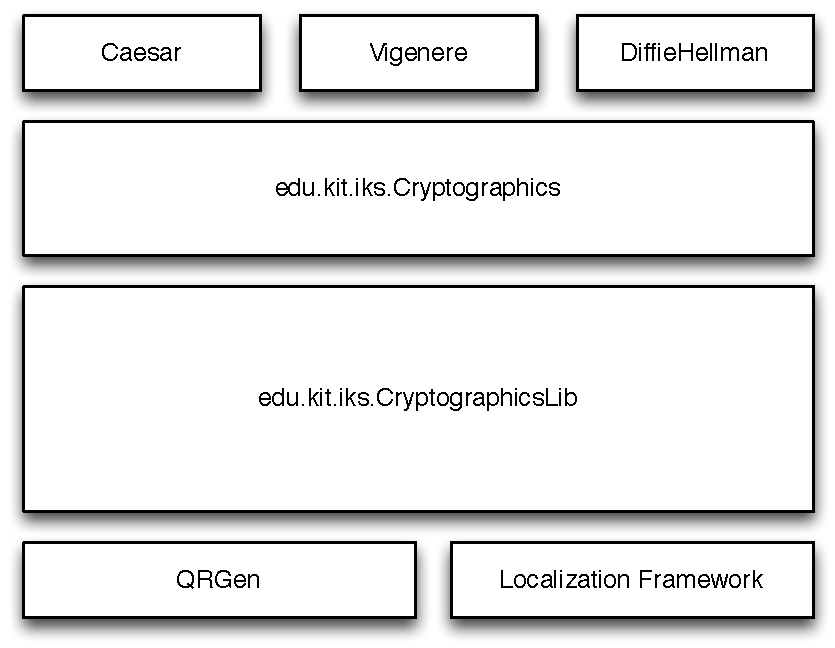
\includegraphics[width=\textwidth]{resources/architecture}
  \caption{Architekturübersicht.}
\end{figure}

In der ersten, der untersten Schicht befinden sich Bibliotheken von Drittanbietern. In unserem Fall handelt es sich hierbei um QRGen, eine Java-Bibliothek um QR-Codes zu generieren, sowie um ein Framework zur Lokalisierung.

In der zweiten Schicht befindet sich das Modul edu.kit.iks.CryptographicsLib. Dieses Modul enthält zum Einen abstrakte Klassen, die von den weiter oben liegenden Klassen verwendet werden. Zum Anderen finden sich hier wiederverwendbare UI-Komponenten, die beispielsweise bei verschiedenen Verfahren verwendet werden können.

Die dritte Schicht besteht aus dem Modul edu.kit.iks.Cryptographics. Hierbei handelt es sich um das Rahmenwerk, in dem alle Visualisierungen ausgeführt werden. Hier wird beispielsweise die Logik implementiert um zwischen Verfahren über eine Zeitleiste wechseln zu können oder auch die Soforthilfe.

Die oberste und vierte Schicht besteht aus den einzelnen, konkreten Verfahren.

Alle Schichten unterteilen ihre Klassen nach dem Model-View-Controller-Prinzip um eine Trennung von Datenmodell, Präsentation und Programmsteuerung zu erreichen. Sowohl die Präsentation als auch die Programmsteuerung verwendet hierbei das Entwurfsmuster Kompositum. Dies erlaubt es uns, eine hierarchische Struktur zu implementieren, und die Aufgaben der Programmsteuerung klar voneinander abzugrenzen. Eine schematische Darstellung der Controller-Hierarchie während einer Visualisierung ist in Abb. 2 zu finden.

\begin{figure}[H]
  \centering
    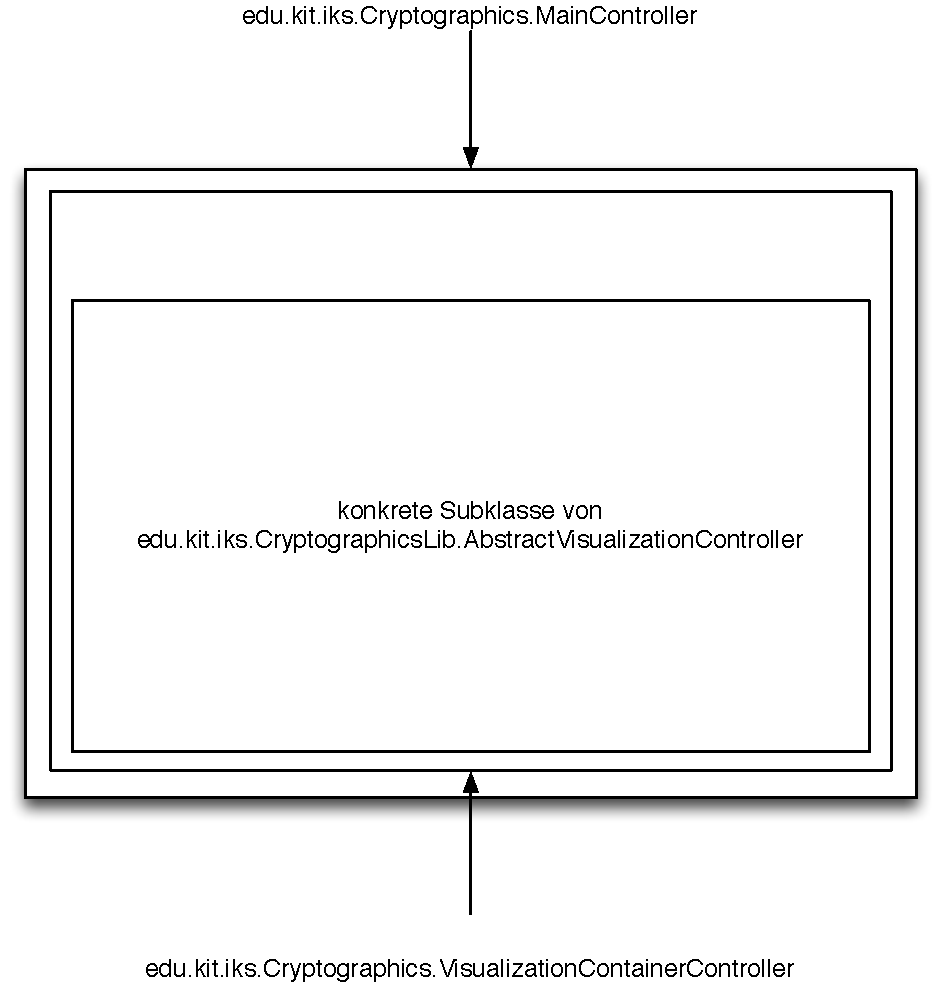
\includegraphics[width=\textwidth]{resources/architecture-2}
  \caption{Darstellung der einzelnen Controller während einer Visualisierung.}
\end{figure}

\section{Klassenbeschreibung}
  \subsection{Paket edu.kit.iks.Cryptographics}
    \subsubsection{Klasse MainController}
      Der MainController erzeugt das Fenster und verwaltet Start- und VisualizationContainerController.
      \begin{figure}[H]
        \centering
        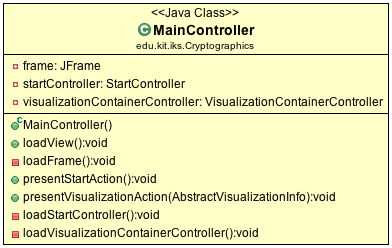
\includegraphics[width=\textwidth]{resources/edu-kit-iks-Cryptographics-MainController}
      \end{figure}

      \textbf{Superklassen und Interfaces}
      \begin{itemize}
        \item edu.kit.iks.CryptographicsLib.AbstractController
      \end{itemize}
      
      \textbf{Methoden}
      \begin{itemize}
        \item public void presentStartAction() \newline
        Lädt den StartController und zeigt seine View an.
      \end{itemize}

  \subsection{Paket edu.kit.iks.CryptographicsLib}
    
    % AbstractController
  	\subsubsection{Klasse AbstractController}
	  Um die MVC-Architektur zu erleichtern wird ein abstrakter Controller benötigt, mit dem Mechanismen
	  für die Controller ausgelagert werden können. Des Weiteren bietet das die Möglichkeit, konkrete
	  Controller mit Hilfe ihrer Substitution anzusprechen.
	
      \begin{figure}[H]
        \centering
        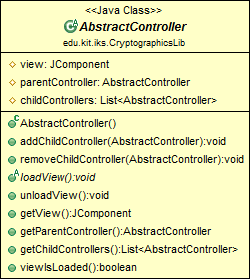
\includegraphics[width=\textwidth]{resources/edu-kit-iks-CryptographicsLib-AbstractController}
      \end{figure}
	
      \textbf{Superklassen und Interfaces}
      \begin{itemize}
        \item \textit{keine}
      \end{itemize}
	
      \textbf{Methoden}
      \begin{itemize}
        \item public void addChildController(AbstractController childController) \newline
          Fügt den übergebenen Kind-Controller zur Liste der Kind-Controller hinzu.
        
        \item public void removeChildController(AbstractController childController) \newline
          Entfernt den übergebenen Kind-Controller aus der Liste der Kind-Controller.
          
        \item abstract public void loadView() \newline
          Abstrakte Deklaration der loadView()-Methode zwingt die erbenden Controller dazu,
          zu definieren, wie ihre View geladen werden soll.
          
        \item public void unloadView() \newline
          Gibt den von der View verbrauchten Speicher wieder frei, sofern diese nicht mehr
          benötigt wird. Zu beachten ist, dass diese Methode über eine Standardimplementierung
          verfügt, es aber durchaus sinnvoll sein kann, das Standardverhalten durch eine
          eigene Implementierung zu überschreiben.
        
        \item public boolean viewIsLoaded() \newline
          Prüft ab, ob die View bereits geladen ist oder nicht.
      \end{itemize}
      
      \textbf{Getter}
      \begin{itemize}
        \item public JComponent getView()
        \item public AbstractController getParentController()
        \item public List<AbstractController> getChildControllers()
      \end{itemize}
      
      \textbf{Setter}
      \begin{itemize}
        \item \textit{keine}
      \end{itemize}
	% /AbstractController
	
	% AbstractVisualizationController
	\subsubsection{Klasse AbstractVisualizationController}
	  Diese abstrakte Klasse konkretisiert den AbstractController zur Verwendung als
	  abstrakter Controller speziell für Visualisierungen. Dies umfasst unter anderem
	  ein Konstruktor, der eine VisualizationInfo als Parameter übergeben bekommt und
	  sich damit initialisiert, sowie einige für Visualisierungen gemeinsame Methoden.
	
      \begin{figure}[H]
        \centering
        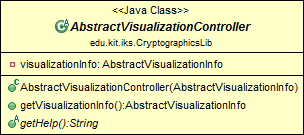
\includegraphics[width=\textwidth]{resources/edu-kit-iks-CryptographicsLib-AbstractVisualizationController}
      \end{figure}
	
      \textbf{Superklassen und Interfaces}
      \begin{itemize}
        \item edu.kit.iks.CryptographicsLib.AbstractController
      \end{itemize}
	
      \textbf{Methoden}
      \begin{itemize}
        \item public AbstractVisualizationController(AbstractVisualizationInfo visualizationInfo) \newline
          Konstruktor. Bekommt als Parameter eine VisualizationInfo, die als Attribut gehalten wird.
        \item abstract public String getHelp() \newline
          Durch das Implementieren dieser Schnittstelle innerhalb eines konkreten Visualisierungs-Controllers
          soll eine einheitliche Hilfe-Funktion geschaffen werden. Dabei muss der konkrete Visualisierungs-
          Controller selbst entscheiden, was die aktuell passende Hilfe ist.
      \end{itemize}
      
      \textbf{Getter}
      \begin{itemize}
		\item public AbstractVisualizationInfo getVisualizationInfo()
      \end{itemize}
      
      \textbf{Setter}
      \begin{itemize}
        \item \textit{keine}
      \end{itemize}
	% /AbstractVisualizationController
	
	% AbstractVisualizationInfo
	\subsubsection{Klasse AbstractVisualizationInfo}
	  Um mit den Metadaten der einzelnen Visualisierungen besser umgehen zu können
	  wird diese Klasse benötigt. Eine konkrete VisualizationInfo muss des Weiteren
	  die abstrakten Methoden implementieren und wird so dazu gezwungen, die 
	  benötigten Metadaten einer Visualisierung bereitzustellen.
	
      \begin{figure}[H]
        \centering
        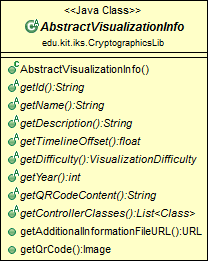
\includegraphics[width=\textwidth]{resources/edu-kit-iks-CryptographicsLib-AbstractVisualizationInfo}
      \end{figure}
	
      \textbf{Superklassen und Interfaces}
      \begin{itemize}
        \item \textit{keine}
      \end{itemize}
	
      \textbf{Methoden}
      \begin{itemize}
        \item abstract public String getId() \newline
          Erzwingt das Setzen einer ID. Die ID wird verwendet, um ein Verfahren anhand
          eines sprechenden Namens identifizieren zu können.
        \item abstract public String getName() \newline
          Erzwingt das Setzen eines Namens. Dieser Name dient als Anzeigename für ein
          Verfahren.
        \item abstract public String getDescription() \newline
          Erzwingt das Setzen einer Beschreibung des Verfahrens. Die Beschreibung ist
          eine Kurzeinleitung und wird zum Beispiel im Popover beim Klicken auf ein
          Verfahren in der Zeitleiste angezeigt.
        \item abstract public float getTimelineOffset() \newline
          Erzwingt das Setzen eines Abstandes auf der Zeitleiste. Dieser Wert liegt
          zwischen 0.0 und 1.0 und ermöglicht eine Sortierung von links (0.0) nach rechts (1.0).
        \item abstract public VisualizationDifficulty getDifficulty() \newline
          Erzwingt das Setzen einer Schwierigkeit die ein enum ist.
        \item abstract public int getYear() \newline
          Erzwingt das Setzen des Jahres, in dem das Verfahren entwickelt wurde.
        \item abstract public String getQRCodeContent() \newline
          Erzwingt das Setzen eines QR-Code-Inhalts. Damit ist der Text gemeint, der
          zu einem QR-Code kodiert werden soll (zum Beispiel eine URL oder eine ISBN).
        \item abstract public List<Class> getControllerClasses() \newline
          Erzwingt das Setzen der Controller, die für die Visualisierung benötigt werden.
          Die Reihenfolge der Klassen in der Liste ist insofern wichtig, als dass dadurch
		  die sequenzielle Reihenfolge beim Abspielen einer Visualisierung definiert wird 
		  (Sprünge sind also trotzdem möglich).
        \item public URL getAdditionalInformationFileURL() \newline
          Gibt die Datei-URL der lokalen HTML-Datei zurück, in der die weiterführenden
          Informationen aufgeführt werden. Diese Methode ist nicht abstrakt, da anhand
          der gesetzten ID ein Standardverzeichnis angesprochen werden kann.
        \item public Image getQrCode() \newline
          Erzeugt ein QR-Code-Bild anhand der gesetzten getQRCodeContent(). Auch diese Methode
          muss nicht abstrakt sein, da es durch die bereits implementierten abstrakten Methoden
          errechnet werden, oder aus dem eventuell vorhandenen Cache geladen werden kann.
      \end{itemize}
      
      \textbf{Getter}
      \begin{itemize}
		\item \textit{keine}
      \end{itemize}
      
      \textbf{Setter}
      \begin{itemize}
        \item \textit{keine}
      \end{itemize}
	% /AbstractVisualizationInfo
	
	% AlphabetStripView
	\subsubsection{Klasse AlphabetStripView}
	  Instanzen dieser Klasse erzeugen eine Zeile mit den Buchstaben des Alphabets.
	  Unter jeder dieser Buchstaben ist eine Durchnummerierung beginnend bei 1 für "A".
	  Eine konkrete Instanz dieser Klasse kann aufgrund ihrer Vaterklasse als JPanel behandelt werden.
	
      \begin{figure}[H]
        \centering
        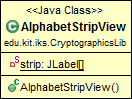
\includegraphics[width=\textwidth]{resources/edu-kit-iks-CryptographicsLib-AlphabetStripView}
      \end{figure}
	
      \textbf{Superklassen und Interfaces}
      \begin{itemize}
        \item javax.swing.JPanel
      \end{itemize}
	
      \textbf{Methoden}
      \begin{itemize}
        \item public AlphabetStripView() \newline
          Konstruktor, der die Alphabetanzeige initialisiert.
      \end{itemize}
      
      \textbf{Getter}
      \begin{itemize}
		\item \textit{keine}
      \end{itemize}
      
      \textbf{Setter}
      \begin{itemize}
        \item \textit{keine}
      \end{itemize}
	% /AlphabetStripView
	
	
	
  \subsection{Paket edu.kit.iks.Cryptographics.Vigenere}
    \subsubsection{Klasse AbstractController}
      Der AbstractController ist eine abstrakte Klasse, die die verschiedenen State-Controller im Vigenere-Paket nutzen.
      \begin{figure}[H]
        \centering
        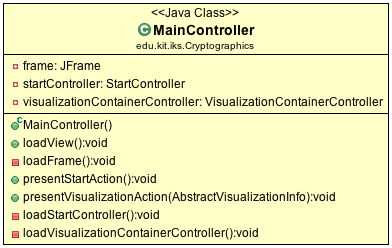
\includegraphics[width=\textwidth]{resources/edu-kit-iks-Cryptographics-MainController}
      \end{figure}

      \textbf{Superklassen und Interfaces}
      \begin{itemize}
        \item edu.kit.iks.CryptographicsLib.AbstractVisualizationController
      \end{itemize}
      
      \textbf{Methoden}
      \begin{itemize}
        \item public String getHelp() \newline
        Gibt den Hilfe-Text an.
        \item public String loadView() \newline
        Lädt die View zum zugehörigen Zustand.
      \end{itemize}

    \subsubsection{Klasse VigenereModel}
      Das VigenereModel ist für die Ver- und Entschlüsselung zuständig.
      \begin{figure}[H]
        \centering
        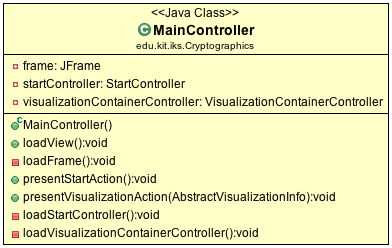
\includegraphics[width=\textwidth]{resources/edu-kit-iks-Cryptographics-MainController}
      \end{figure}
      
      \textbf{Methoden}
      \begin{itemize}
        \item public char XOR(char a, char b) \newline
        Benutzt einen logischen XOR auf die Parameter a und b.
      \end{itemize}

    \subsubsection{Klasse VigenereVisualizationInfo}
      VigenereVisualizationInfo enthält alle wichtigen Informationen zu dem Verfahren, wie z.B. Verfahrensname/Beschreibung.
      \begin{figure}[H]
        \centering
        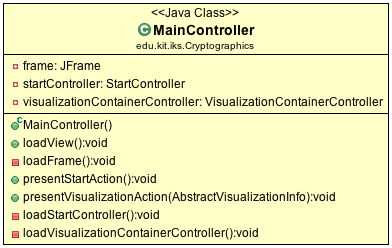
\includegraphics[width=\textwidth]{resources/edu-kit-iks-Cryptographics-MainController}
      \end{figure}

      \textbf{Superklassen und Interfaces}
      \begin{itemize}
        \item edu.kit.iks.CryptographicsLib.AbstractVisualizationInfo
      \end{itemize}
      
      \textbf{Methoden}
      \begin{itemize}
        \item public String getId() \newline
        Gibt die Kennungs-ID aus.
        \item public String getName() \newline
        Gibt den Namen des Verfahrens aus.
        \item public String getDescription() \newline
        Gibt die Beschreibung des Verfahrens aus.
        \item public String getQRCodeContent() \newline
        Gibt den Inhalt des QRCodes aus.
        \item public float getTimelineOffset() \newline
        Gibt die relative Position in der Timeline aus.
        \item public VisualizationDifficulty getDifficulty() \newline
        Gibt den Schwierigkeitsgrad aus.
        \item public int getYear() \newline
        Gibt das Jahr aus, in welchem das Verfahren entwickelt wurde.
        \item public List<Class> getControllerClasses() \newline
        Gibt eine Liste von Controller-Klassen des Verfahrens aus, welche dann im Statecontroller geswitcht werden können.
      \end{itemize}

  \subsection{Paket edu.kit.iks.Cryptographics.Vigenere.Demonstration}
    \subsubsection{Klasse FirstDemonstrationController}
      Der FirstDemonstrationController erstellt FirstDemonstrationView.
      \begin{figure}[H]
        \centering
        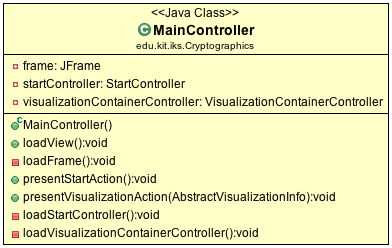
\includegraphics[width=\textwidth]{resources/edu-kit-iks-Cryptographics-MainController}
      \end{figure}

      \textbf{Superklassen und Interfaces}
      \begin{itemize}
        \item edu.kit.iks.CryptographicsLib.AbstractController
      \end{itemize}

    \subsubsection{Klasse FirstDemonstrationView}
      Die FirstDemonstrationView zeigt die Informationen über Vigenere sowie eine kurze Erklärung über Modulo.
      \begin{figure}[H]
        \centering
        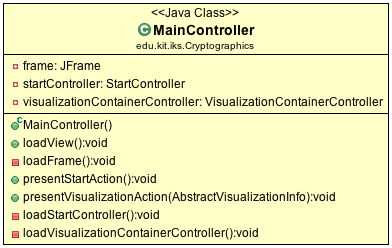
\includegraphics[width=\textwidth]{resources/edu-kit-iks-Cryptographics-MainController}
      \end{figure}

      \textbf{Superklassen und Interfaces}
      \begin{itemize}
        \item edu.kit.iks.CryptographicsLib.VisualizationView
      \end{itemize}

    \subsubsection{Klasse SecondDemonstrationController}
      Der SecondDemonstrationController erstellt SecondDemonstrationView.
      \begin{figure}[H]
        \centering
        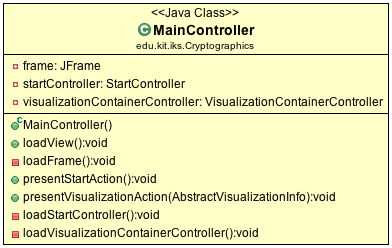
\includegraphics[width=\textwidth]{resources/edu-kit-iks-Cryptographics-MainController}
      \end{figure}

      \textbf{Superklassen und Interfaces}
      \begin{itemize}
        \item edu.kit.iks.CryptographicsLib.AbstractController
      \end{itemize}

    \subsubsection{Klasse SecondDemonstrationView}
      Die SecondDemonstrationView zeigt eine Animation über die Funktionsweise der Verschlüsselung mit Vigenere.
      \begin{figure}[H]
        \centering
        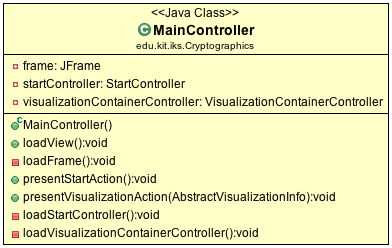
\includegraphics[width=\textwidth]{resources/edu-kit-iks-Cryptographics-MainController}
      \end{figure}

      \textbf{Superklassen und Interfaces}
      \begin{itemize}
        \item edu.kit.iks.CryptographicsLib.VisualizationView
      \end{itemize}

    \subsubsection{Klasse ThirdDemonstrationController}
      Der ThirdDemonstrationController erstellt ThirdDemonstrationView.
      \begin{figure}[H]
        \centering
        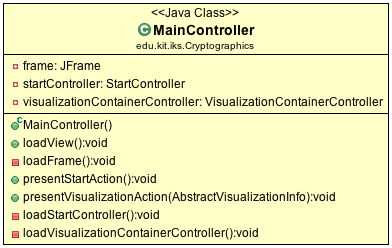
\includegraphics[width=\textwidth]{resources/edu-kit-iks-Cryptographics-MainController}
      \end{figure}

      \textbf{Superklassen und Interfaces}
      \begin{itemize}
        \item edu.kit.iks.CryptographicsLib.AbstractController
      \end{itemize}

    \subsubsection{Klasse ThirdDemonstrationView}
      Die ThirdDemonstrationView zeigt eine Animation über die Funktionsweise der Entschlüsselung mit Vigenere.
      \begin{figure}[H]
        \centering
        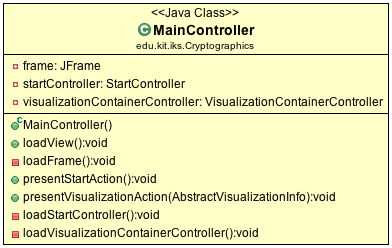
\includegraphics[width=\textwidth]{resources/edu-kit-iks-Cryptographics-MainController}
      \end{figure}

      \textbf{Superklassen und Interfaces}
      \begin{itemize}
        \item edu.kit.iks.CryptographicsLib.VisualizationView
      \end{itemize}

\subsection{Paket edu.kit.iks.Cryptographics.Caesar}
\subsection{Paket edu.kit.iks.Cryptographics.DiffieHellman}

\section{Abläufe}

\section{Entwurfdaten}

\section{Anhang}
\glsaddall
\printglossary[numberedsection, style=altlist]

\end{document}
